\documentclass[preprintnumbers,amsmath,amssymb,onecolumn,12pt]{revtex4}
\usepackage{graphicx}% Include figure files
\usepackage{dcolumn}% Align table columns on decimal point
\usepackage{bm}% bold math
\usepackage{natbib}
\usepackage{physics}
\usepackage[caption=false]{subfig}

\def\sgn{\mathop{\rm sgn}}

\begin{document}

\vspace{0.2in}
{\Large \hspace{1.6in}\textsc{Supplementary Material} }\\
\
\title{Mechanical Detection of Dipole-Dipole Interactions \\between Electronic Spins in a Solid}

\author{C. Pellet-Mary, P. Huillery, M. Perdriat, G. H\'etet} 


\affiliation{$^1$
Laboratoire de Physique de l'Ecole normale sup\'erieure, ENS, Universit\'e PSL, CNRS, Sorbonne Universit\'e, Universit\'e Paris-Diderot, Sorbonne Paris Cit\'e, Paris, France.
}

\begin{abstract}
\end{abstract}

\maketitle

\tableofcontents

\newpage

\section*{NV$^-$ center Theory}
\subsection{NV spin Hamiltonian}
The NV spin Hamiltonian in its fundamental level can be written as :
\begin{equation*}
  \hat{\mathcal{H}}_s=D S_z^2 + \gamma_e \textbf{B}\cdot\hat{\textbf{S}},
  \end{equation*} 
Where $D = (2\pi) 2.87$ GHz is the crystal field splitting and $\gamma_e = 28 $GHz/T is the electron gyromagnetic ratio. We neglected contributions of the strain and local electric field since we are working with magnetic fields of the order of 100G, as well as the hyper-fine interaction with $^{14}$N since we are working with ensembles with a typical inhomogeneous broadening $\frac{1}{T_2^*} = (2\pi) 5$ MHz.

The \textbf{z} axis of the $S_z$ operator here is the axis formed by the nitrogen atom and the vacancy, hence why we do have different energy transitions for different NV orientations, depending on the projection of the magnetic field on the NV axis.

\subsection{Diamond crystalline axes and degeneracy conditions}
\begin{figure}[!ht]
  \centering \scalebox{0.45}{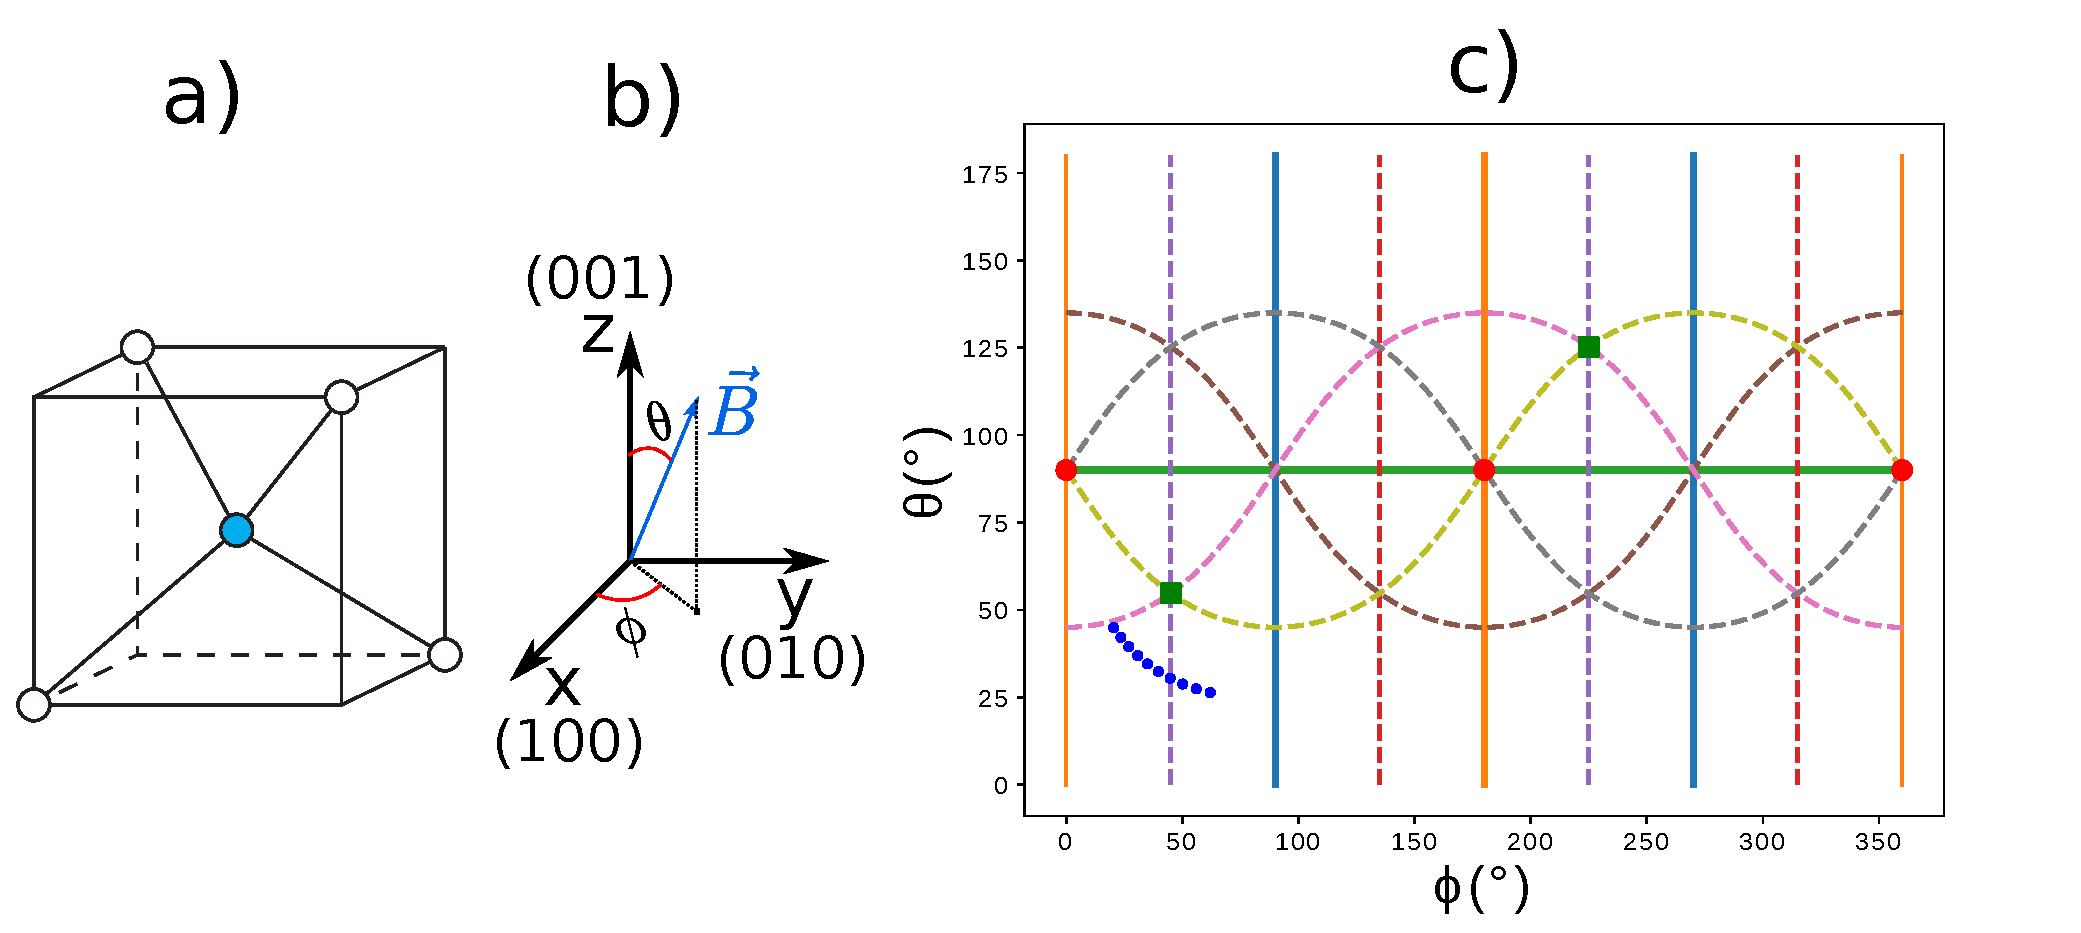
\includegraphics{SI_Cristallo}}
  \caption{Representation of the magnetic field in the diamond crystalline basis.}
	\label{cristallo}
\end{figure}
There are four possible crystalline axis for the NV centers (so-called "classes" of NV) which are depicted in Fig. \ref{cristallo} b) and correspond to the crystalline directions [$111$], [$1\bar 1 \bar 1$], [$\bar 1 1 \bar 1$] and [$\bar 1 \bar 1 1$]. 

The magnetic field is represented in the diamond basis in Fig. \ref{cristallo} a) where the usual polar and azimuthal angles $\theta$ and $\phi$ are defined with respect to the \textbf{z} ([$001$]) direction.

For some orientations of the magnetic field, the projection of the magnetic field on two or more NV axes will be identical, and therefore the energy level of the corresponding classes will be the same. These degeneracies are represented on fig \ref{cristallo} c), where the dashed lines are the locus of the crystalline planes orthogonal to the [110] directions (6 planes in total). When the magnetic field belongs to these plane, we observe a degeneracy between two classes of NV, as can be seen in the Fig. 4 of the main paper.

The plain lines are the locus of the planes orthogonal to the [100] directions (3 planes total). When the magnetic field is in these planes, every class is at resonance with another class, as can be seen in Fig. X.

The red circles correspond to the [100] directions, for which the four classes of NV or at degeneracy, and the green squares to the [111] direction where one class is aligned with the magnetic field, and the three other are at degeneracy.

Finally the blue dots correspond to the path followed by the magnetic field in the experiment presented in Fig 4. of the main text, where we can see a degeneracy plane of the [110]$_\perp$ family being crossed.

\section*{Experimental details}

\subsection{Experimental setup}

\begin{figure}[!ht]
  \centering \scalebox{0.3}{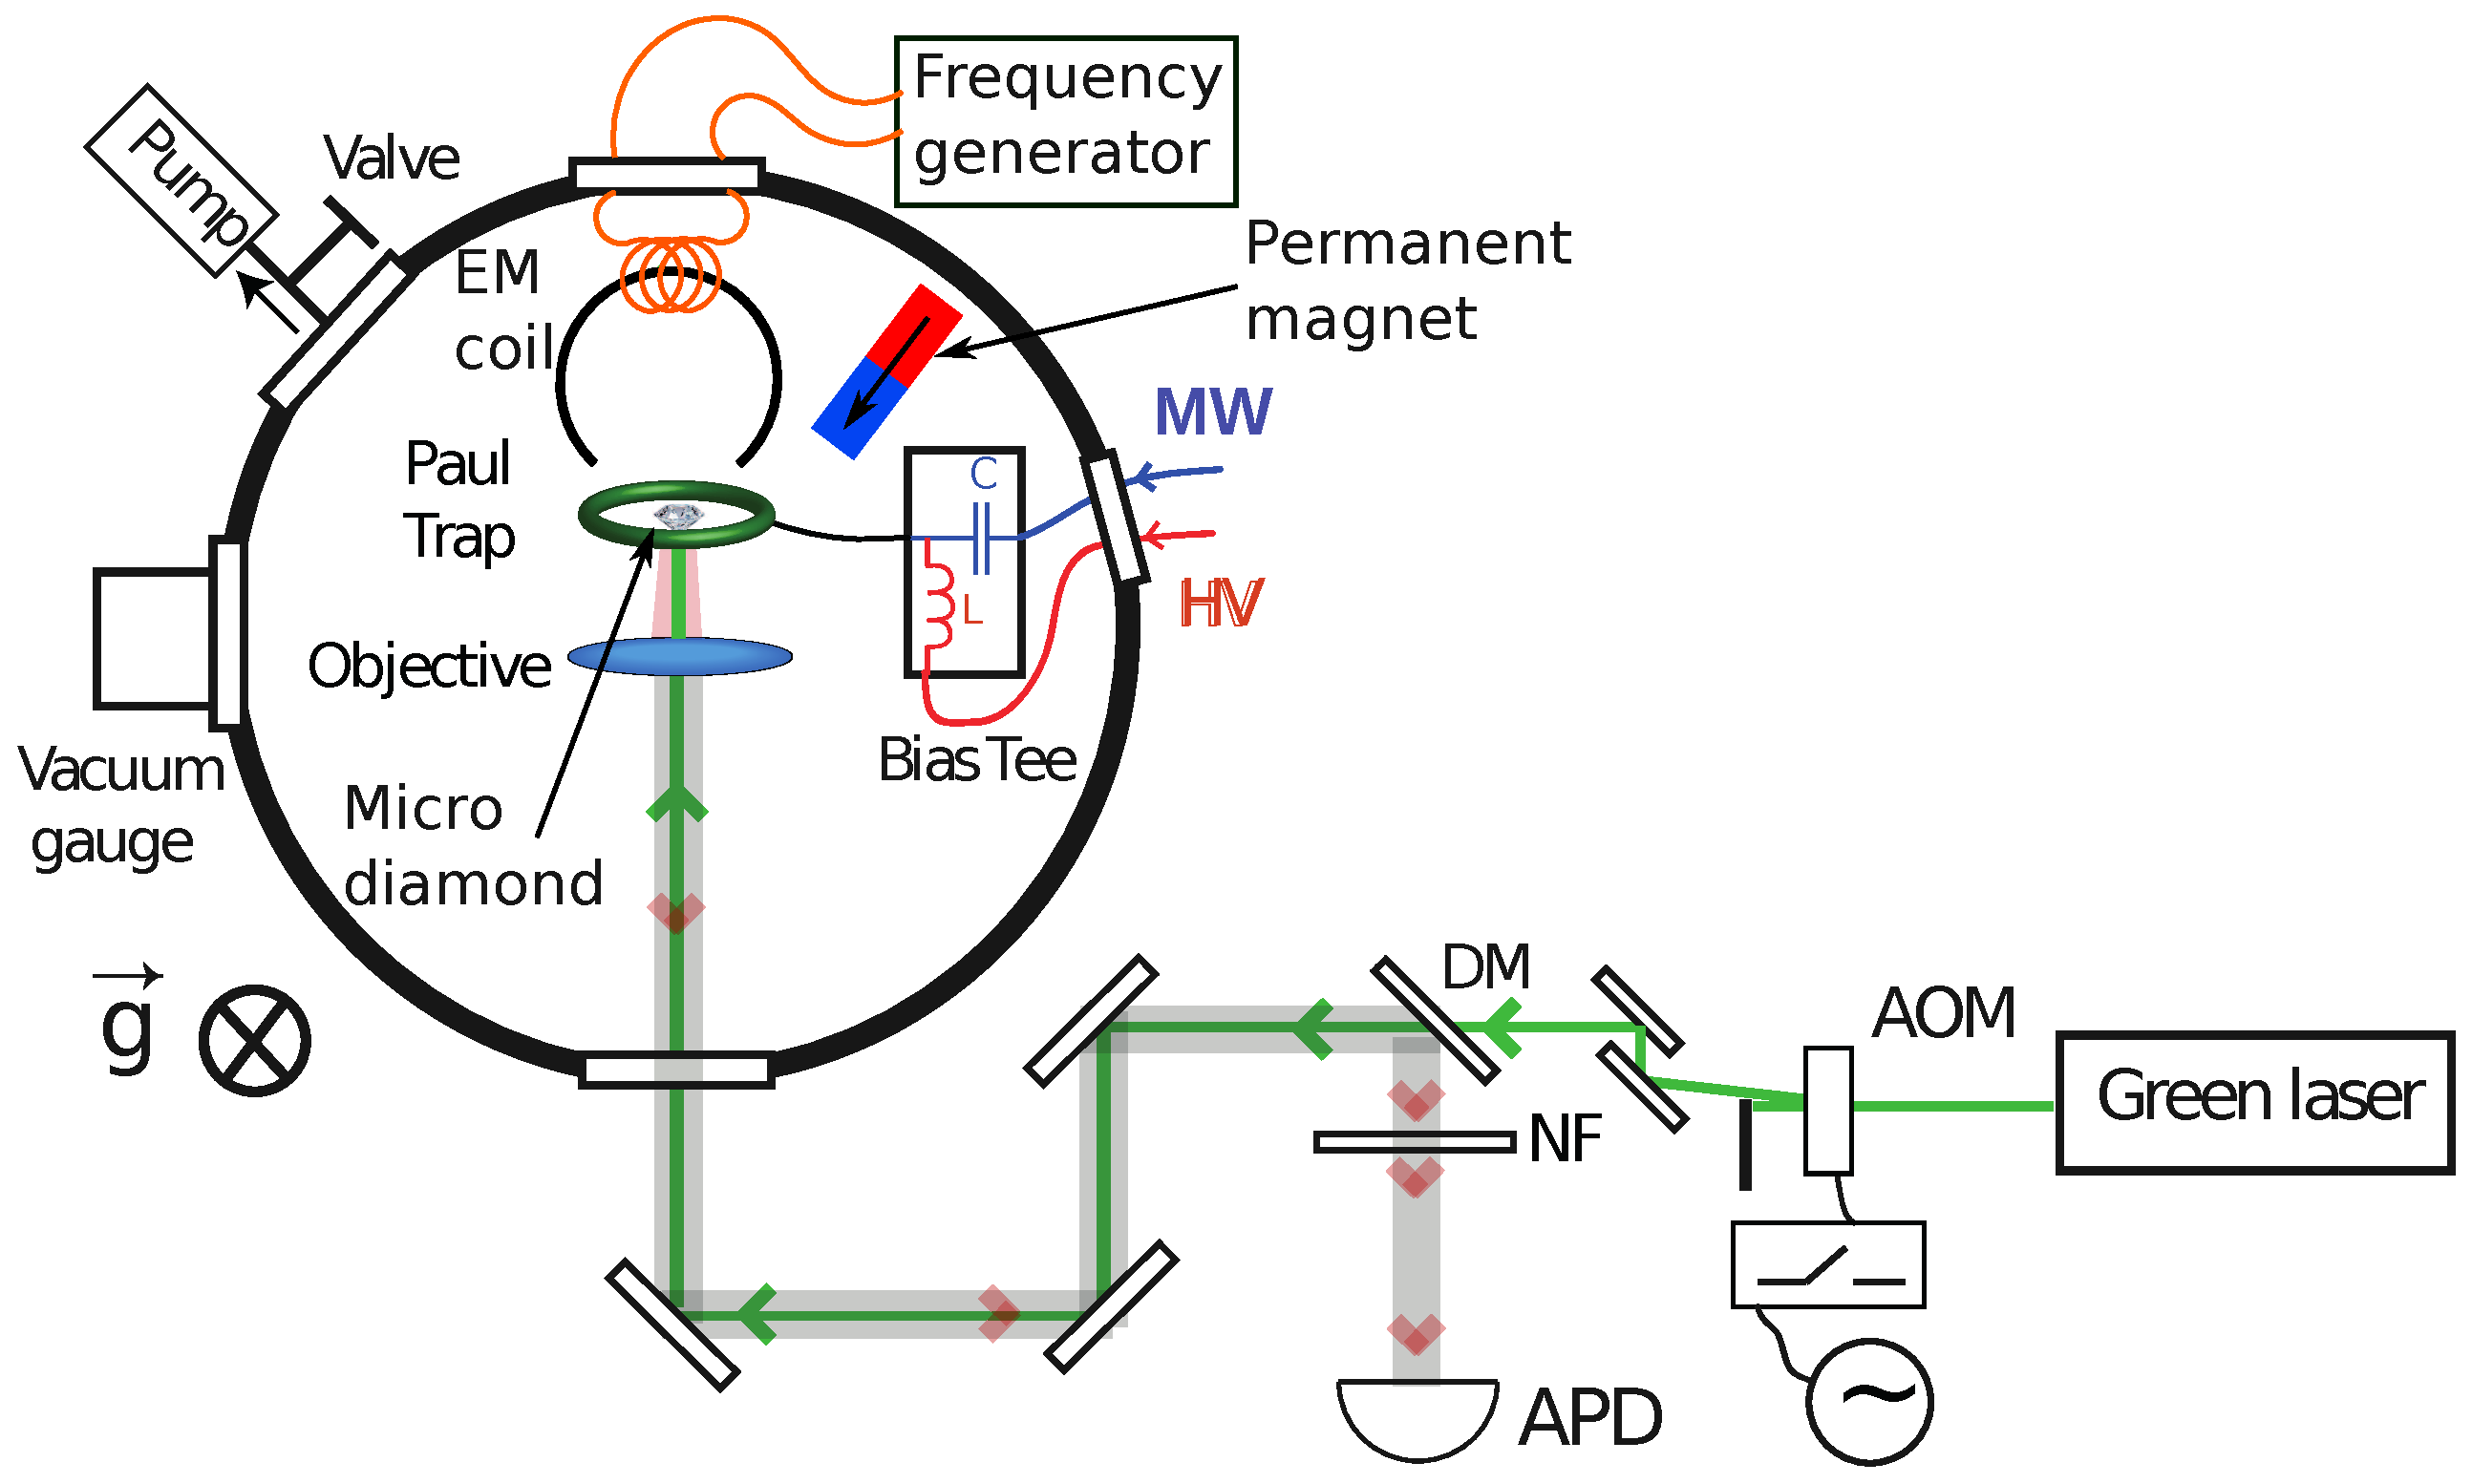
\includegraphics{setup}}
  \caption{Illustration of the experimental setup}
	\label{Optics}
\end{figure}

The experimental setup illustrated in Fig.\ref{Optics} is very similar to the one used in \citep{DelordPRL} with the addition of a permanent magnet and an electromagnetic (EM) coil in order to perform magnetic filed scans. The diamond sample is typically illuminated with 1mW of 532 nm laser light, focused by a NA = 0.5 objective. An acousto-optic modulator (AOM) is used to switch on and off the 532nm laser and to finely tuned its power. The photo-luminescence (PL) is collected by the objective, separated form the excitation light using a dichroic mirror (DM) and a 532nm notch filter (NF), and detected using a multimode-fibered single-photon avalanche photo-detector (APD) (SPCM-AQRH-15 from Perkin Elmer). Typically, we detect PL photons at a rate of 1MHz. 

The Paul trap is a pseudo-ring as can be seen in \citep{DelordPhD} which acts both as trap through the high voltage (HV) and as a microwave (MW) antenna.

The magnetic field generated by the (homemade) EM coil is controlled by a frequency generator (HP 33120A) with a triangle signal in order to perform magnetic field ramps. For scans of less than 100 G, no amplification of the signal is required.

While the levitating setup is located in a vacuum chamber, all the experiments presented in this article are performed at atmospheric pressure.


\subsection{$T_1$ Measurement}
\begin{figure}[!ht]
  \centering \scalebox{1}{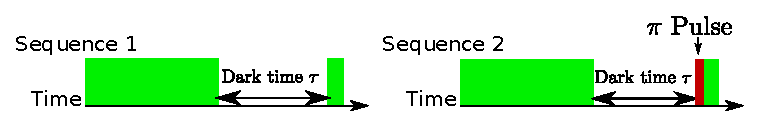
\includegraphics{T1_soustraction_shema}}
  \caption{T$_1$ measurement protocol for a single class in an ensemble of NV centers}
	\label{T1_protocol}
\end{figure}
The protocol to measure the spin lifetime of the NV centers, as presented in Fig 2. of the main text, is described in Fig. \ref{T1_protocol} . The spins are initially polarized in their $m_s=\ket{0}$ state through a 1 ms green laser excitation pulse and then left to evolve in the dark for a variable dark time $\tau$. The spin state is finally read out with a 10 $\mu$s laser pulse, shorter than the polarization time of the spins.

The sequence is repeated a second time, adding a resonant microwave $\pi$ pulse on a transition of one of the four classes of NV$^-$, exchanging the population of the $m_s=\ket{0}$ state with one of the $m_s=\ket{\pm 1}$ state.

The two sequences are then subtracted, allowing us to measure the spin state population of a single class, and removing unwanted contributions to the photoluminescence, such as charge state transfer in the dark.

\subsection{Magnetic field calibration}

A permanent magnet is placed a few cm away from the diamond sample in order to apply a uniform magnetic field to the NV centers together with an electro-magnet.

To calibrate the magnetic field magnitude $B$, and its orientation $\theta$ with respect to the NV axis, we record Optically Detected Magnetic Resonace (ODMR) spectra.... 



\subsection{Spin-mechanical detection}

The microwave detuning is scanned in 2~MHz steps with a duration of 10 ms per points. During those 10ms, the diamond orientation has enough time to reach its equilibrium position and the spin torque effect can be observed. The average count-rate is about 1 MCounts/s.

\subsection{PL detection}

In these measurements, compared to \cite{DelordNat}, to detect the PL we use another detection channel that is more resilient to motion. We therefore do not need to detect prior to ring down.

\section*{Cross-relaxation detection for another type of degeneracy}

\section*{Simulation details}
In this part we will discuss the method used to simulate the average torque as well as the $\ket{m_s=0}$ population of the stationary state. The numerical solving of the master equations was performed thanks to Quantum Toolbox in Python (QuTiP) \citep{qutip1} \citep{qutip2}.

In order to describe the dynamics of our spin ensemble, besides the spin Hamiltonian described in the first part, we introduce the incoherent optical pumping through the jump operators $\mathcal{L}_+ = \Gamma_l \ket{0}\bra{+1} $ and $\mathcal{L}_- = \Gamma_l \ket{0}\bra{-1} $, where $\Gamma_l \approx (2\pi) 10$kHz is the polarizing rate due to the laser.

We also introduce the usual T1 jump operators...

In order to describe the T1 modification induced by the cross-relaxations, we use a phenomenological model ...

According to previous measurements \citep{choi_depolarization_2017}, only the $\ket{0}\bra{\pm1}$ (corresponding to a single quantum exchange in the dipole-dipole interaction) operators are modified by the cross-relaxations.

\bibliography{trap}

\end{document}
